\begin{figure}[H]
    \centering
    \definecolor{massred}{RGB}{185,55,45}
    \definecolor{sphereblue}{RGB}{100,165,215}
    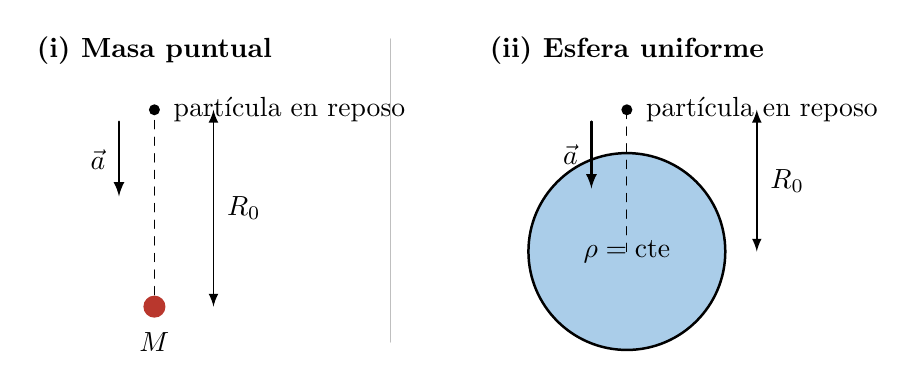
\begin{tikzpicture}[x=1cm,y=1cm,line cap=round,line join=round]
        % Masa puntual
        \node[font=\bfseries] at (3.0,4.00) {(i) Masa puntual};
        \fill[massred] (3.0,0.75) circle (0.14);
        \node[below] at (3.0,0.55) {$M$};
        \fill (3.0,3.25) circle (0.07);
        \node[right] at (3.12,3.25) {partícula en reposo};
        \draw[dashed] (3.0,0.90) -- (3.0,3.18);
        \draw[-latex,line width=0.8pt] (2.55,3.10) -- (2.55,2.15);
        \node[left] at (2.50,2.62) {$\vec a$};
        \draw[latex-latex,line width=0.6pt] (3.75,0.75) -- (3.75,3.25);
        \node[right] at (3.80,2.00) {$R_0$};

        % Separador
        \draw[black!25] (6.0,0.30) -- (6.0,4.15);

        % Esfera uniforme
        \node[font=\bfseries] at (9.0,4.00) {(ii) Esfera uniforme};
        \fill[sphereblue!55] (9.0,1.45) circle (1.25);
        \draw[line width=0.9pt] (9.0,1.45) circle (1.25);
        \node at (9.0,1.45) {$\rho=\mathrm{cte}$};
        \fill (9.0,3.25) circle (0.07);
        \node[right] at (9.12,3.25) {partícula en reposo};
        \draw[dashed] (9.0,1.45) -- (9.0,3.18);
        \draw[-latex,line width=0.8pt] (8.55,3.10) -- (8.55,2.25);
        \node[left] at (8.50,2.68) {$\vec a$};
        \draw[latex-latex,line width=0.6pt] (10.65,1.45) -- (10.65,3.25);
        \node[right] at (10.70,2.35) {$R_0$};
    \end{tikzpicture}
    \caption{Comparación de la caída hacia una masa puntual y hacia una esfera uniforme.}
\end{figure}